\chapter{Processamento de Linguagem Natural}
\label{cap:Processamento}

% Um computador, obviamente, está preparado para entender sua própria linguagem,
% como por exemplo, um compilador interpreta linhas de código fonte para gerar um
% programa executável seguindo exatamente o algoritmo utilizado. Por isso, temos o
% termo Natural no Processamento de Linguagem.

O objetivo da área de Processamento de Linguagem Natural é analisar a linguagem natural, ou seja, a linguagem utilizada pelo seres humanos não
importando se essa é escrita ou falada \cite{manningschutze1999}.

O Processamento de Linguagem Natural é uma área antiga, sendo anterior a
invenção dos computadores modernos. De fato, sua primeira grande aplicação foi
um dicionário desenvolvido no Birkbeck College em Londres no ano de 1948. Por ser
uma área complexa, seus primeiros trabalhos foram notavelmente falhos o que
causou uma certa hostilidade por parte das agências formentadoras de pesquisas.

Os primeiros pesquisadores eram muitas vezes bilíngues, como por exemplo,
nativos alemães que imigraram para os Estados Unidos. Acreditava-se que pelo
fato desses terem conhecimento de ambas as linguas, Ingles e Alemão, eles teriam
capacidade de desenvolver programas de computadores que efetuariam a tradução das linguas
de modo satisfatório. Uma vez que esses encontraram muitas dificuldades,
ficou claro que o maior problema não era o conhecimento de ambas as
línguas e sim como expressar esse conhecimento na forma de um programa de
computador \cite{history}.

Para que um computador seja capaz de interpretar uma
língua, necessitamos antes entender como nós efetuamos essa
interpretação.
Por isso, uma parte considerável do Processamento de Linguagem Natural está apoiado na área de Linguística.

\section{Linguística}

O objetivo da Linguística é compreender como os humanos adquirem, produzem e
entendem as diversas línguas, ou seja, a forma com que conversamos, a nossa
escrita e outras mídias de comunicação \cite{manningschutze1999}.

Na linguagem tanto escrita, como na falada, existem regras que são utilizadas
para estruturar as expressões. Uma série de dificuldades no Processamento de
Linguagem Natural são ocasionadas pelo fato de que as pessoas constantemente
mudam essas regras para satisfazerem suas necessidades de comunicação
\cite{manningschutze1999}. Uma vez que as regras são constantemente modificadas pelo loucutor, se torna extremamente difícil a criação de um software ou hardware efetue a interpretação de uma língua.


% \subsection{Sintaxe e Semântica}
%
% No seu livro Estruturas Sintáticas, Noam Chomsky cita as seguintes frases
% ``Ideias verdes incolores dormem furiosamente'' e ``Incolores verde ideias dormem
% furiosamente''.
%
% A primeira frase, do ponto de vista sintático é correta, porém, assim como a
% segunda frase, semânticamente não faz sentido.
%
% O fato de que podemos modificar as regras da lingua de duas formas distintas é
% utilizado como evidência para a separação da sintaxe e semântica na língua.
% \cite{jacksonmoulinier2007}

\section{Métodos de Processamento de Linguagem Natural}

O \ac{NLP} tem como objetivo a execução de diferentes tarefas, como por exemplo,
a categorização de documentos, a tradução e a geração de textos a partir de um
banco de dados, etc. Podemos citar duas classes de métodos para a execução deste
tipo de tarefas, que são os métodos simbólicos e os métodos estatísticos.

Nos final dos anos 50 e 60, existiam excelentes métodos esatatísticos, que foram
desenvolvidos durante a segunda guerra mundial, para a solução de problemas
científicos \cite{shannon48}.
Porém, no ano de 1957, Chomsky publicou o trabalho intitulado de
\textit{``Syntactic Structures''} onde descreve a
teoria de gramática gerativa, que considera a gramática como um conjunto de regras. Essa abordagem através de um
conjunto de regras, ao invés de um modelo matemático, entra em conflito com os
trabalhos anteriores, criando duas comunidades no campo de Linguística. Como
reflexo dessas duas comunidades, a área de \ac{NLP} que crescia em paralelo a
linguística também foi dividida em duas áreas. A primeira dessas áreas que fazia
uso de métodos baseados em regras (simbólico) e a segunda que fazia o uso de
métodos quantitativos (estatísticos).


Nesta seção será apresentado um exemplo de método simbólico e de um método
estatístico.
Destaca-se que essa descrição apresenta como objetivo somente diferenciar
ambas as classes de métodos, através de seus requisitos e forma de execução.
Destaca-se ainda que os métodos apresentados não são utilizados na
análise de sentimentos, sendo que os métodos específicos que são utilizados para
identificação de sentimentos serão descritos no Capítulo \ref{cap:Classificadores}.


\subsection{Método Simbólico}
O método simbólico ou racionalista está
baseado no campo da Linguística e faz o uso da manipulação dos símbolos,
significados e das regras de um texto. Um exemplo de método simbólico é o
método de Brill \cite{Brill:1992:SRP:974499.974526}. Por exemplo, no método de
Brill a frase ``João pintou a casa de branco'', será separada em palavras que
serão classificadas através de um dicionário pré-definido, como:

\begin{table}[htb]
\centering
\begin{tabular}{l|l|l|l|l|l|l}
Palavra         & João        & pintou & a      & casa        & de
& branco
\\
%Correta: & Substantivo & Verbo  & Artigo & Substantivo & Preposição &
% Substantivo \\
Classificação:   & 			   & Verbo  & Artigo & Substantivo & Preposição & Adjetivo
\end{tabular}
\label{my-label}
\end{table}

Observa-se que algumas palavras não foram
identificadas, como ``João'' ou classificadas de forma incorreta, como
``branco". Desta forma, o método utiliza-se de outras duas regras para a
classificação.
A primeira regra classifica todas as palavras desconhecidas que iniciam em
maiúsculo como substantivos, por exemplo, a palavra ``João''. Já a segunda regra, atribui para a palavra desconhecida a mesma classificação
de outras palavras que terminam com as mesmas três letras. Por exemplo, supondo
que a palavra ``pintou'' não fosse encontrada no dicionário, essa seria
associada a outras palavras terminadas com o sufixo ``tou'', ou seja, essa seria
classificada como verbo.

\begin{table}[htb]
\centering
\begin{tabular}{l|l|l|l|l|l|l}
Palavra         & João        & pintou & a      & casa        & de
& branco
\\
%Correta: & Substantivo & Verbo  & Artigo & Substantivo & Preposição &
% Substantivo \\
Classificação:   & \textbf{Substantivo} & Verbo  & Artigo & Substantivo &
Preposição & Adjetivo
\end{tabular}
\label{my-label}
\end{table}



Após essa classificação inicial, o método executa o seguinte conjunto de
regras, ou ainda, regras derivadas dessas:

\begin{itemize}
  \item Se uma palavra tem a classificação \textbf{A} e está no contexto
  \textbf{C} então a sua classificação deverá ser mudada para \textbf{B}. Por
  exemplo, se uma palavra \textbf{A} (branco no exemplo) é um adjetivo e uma das
  duas palavras anteriores é uma preposição (``de'' no contexto \textbf{C}
  ), mude para sua classificação para substantivo (classificação \textbf{B}).
  
  \[\overbrace{\text{João}}^\text{Substantivo}
  \overbrace{\text{pintou}}^\text{Verbo}
  \overbrace{\text{a}}^\text{Artigo}
  \underbrace{
  \overbrace{\text{casa}}^\text{Substantivo}
  \overbrace{\text{de}}^\text{Preposição}}_\text{Contexto \textbf{C}}
  \underbrace{\overbrace{\text{branco}}^{\textcolor{red}{Adjetivo}}}_\text{Classificação
  \textbf{A}\textrightarrow\textbf{B}}
  \]
  
  \item Se uma palavra tem a classificação \textbf{A} e tem uma propriedade
  \textbf{P} então a sua classificação deverá ser alterada para \textbf{B}. Por
  exemplo, se uma palavra \textbf{A} (``Linda'') foi classificada como um
  adjetivo e é iniciada com uma letra maiúscula (propriedade \textbf{P}), sua
  classificação deverá ser alterada para substantivo (classificação \textbf{B}).
  
  \[\overbrace{\text{Comprei}}^\text{Verbo}
  \overbrace{\text{flores}}^\text{Substantivo}
  \overbrace{\text{para}}^\text{Preposição}
  \underbrace{\overbrace{\text{L}\text{inda}}^{\textcolor{red}{Adjetivo}}}_\text{Classificação
  \textbf{A}\textrightarrow\textbf{B}}
  \]
  
  \item Se uma palavra tem a classificação \textbf{A} e uma palavra com a
  propriedade \textbf{P} está na região \textbf{R}, sua classificação deverá
  ser \textbf{B}. Por exemplo, se uma das duas palavras anteriores (``João
  adora" na região \textbf{R}) iniciam com letra maiúscula (propriedade
  \textbf{P}), sua classificação deverá ser alterada para substantivo (classificação \textbf{B}).
  
  \[\underbrace{\overbrace{\text{João}}^\text{Substantivo}
  \overbrace{\text{adora}}^\text{Verbo}}_\text{Região \textbf{R}}
  \underbrace{\overbrace{\text{L}\text{inda}}^{\textcolor{red}{Adjetivo}}}_\text{Classificação
  \textbf{A}\textrightarrow\textbf{B}}
  \]
  
  
\end{itemize}

\subsection{Método Estatístico}
Um método estatístico utiliza-se de uma grandes
quantidade de texto, procurando por padrões e
associações a modelos, sendo que esses padrões podem ou não estar relacionados
com regras sintáticas ou semânticas.

Os métodos estatísticos baseia-se na utilização de um sistema de aprendizado
supervisionado, ou seja, a classificação é feita a partir de um conjunto de dados já
classificado, que é chamado de \textit{training set}. Um exemplo de método
estatístico é a utilização de Modelos de Markov com a aplicação do algoritmo de
Viterbi \cite{manningschutze1999}.

Em um Modelo de Markov, a classificação da frase ``João comprou um
carro" é feita a partir de um \textit{training set} que pode, por exemplo, ser
composto por textos retirados de \textit{web-sites}, sendo que as palavras
destes textos já devem estar classificadas. A partir deste \textit{training
set}, as palavras ``João'', ``comprou'' e ``carro'' seriam classificadas como
substantivo, verbo e substantivo, respectivamente. Já a palavra ``um'' apresenta uma ambiguidade uma vez que pode
ser classificada como um artigo (ART), ou um substantivo (SM) ou um pronome
(PRO).
A Figura \ref{fig:markov} representa o conjunto de possibilidades que o
classificador pode utilizar para a classificação completa da frase.

\begin{figure}[htbp]
\centering
\includegraphics[height=180px]{imagens/markov.png}
\caption{Caminhos possíveis de classificação}
\label{fig:markov}
\end{figure}

A idéia central da utilização de Modelos de Markov é
escolher, entre esses caminhos (Figura \ref{fig:markov}), o caminho de maior
probabilidade. Para tanto, se faz necessário calcular a probabilidade de todos
os caminhos seguindo o Modelo de Markov e após este cálculo, utilizar o
Algoritmo de Viterbi para definir qual caminho é o mais provável.

O Modelo de Markov irá utilizar-se do \textit{training set} para inferir a
classificação da palavra ``um''. Para este exemplo, vamos considerar um
\textit{training set} hipotético com as seguintes características: 10000
Substantivos aonde 150 são a palavra ``um'', 10
são a palavra ``João'' e 50 são a palavra ``carro'', 20000 Artigos aonde 500 são
a palavra ``um'', 12000 Verbos aonde 50 são a palavra ``comprou'' e 15000
Pronomes aonde 50 são a palavra ``um''. Neste caso, a probabilidade da palavra
ser um substantivo é dada pela equação:

\[ P(palavra|classe) = \frac{C(classe,palavra)}{C(classe)} \]

\[ P(um|SM) = \frac{C(SM,um)}{C(SM)} = \frac{150}{10000} = 0.015 \]

Da mesma forma, é calculada a probabilidade de ``um'' pertencer as demais
classes, neste caso, pronome ou artigo. Por exemplo, a probabilidade da palavra
``um'' ser um pronome seria 0.0033 e a probabilidade da palavra ``um'' ser um
artigo seria 0.025. Esse cálculo é realizado para todas as palavras da frase
que está sendo classificada e todas as classes possíveis. A Tabela
\ref{tabela:associacao} apresenta o cálculo realizado anteriormente para as
demais palavras e classes.

\begin{table}[htb]
\centering
\begin{tabular}{|l|l|l|l|l|}
\hline
& João  & comprou & um     & carro  \\ \hline
Substantivo & 0.001 & 0       & 0.015  & 0.005  \\ \hline
Verbo       & 0     & 0.0042  & 0      & 0      \\ \hline
Artigo      & 0     & 0       & 0.025  & 0      \\ \hline
Pronome     & 0     & 0       & 0.0033 & 0      \\ \hline
\end{tabular}
\caption{Tabela de Probabilidades de Associação}
\label{tabela:associacao}
\end{table}

Além da probabilidade de associação a uma determinada classe, é calculada a
probabilidade de transição de uma classe para a outra. Neste caso, o
\textit{training set} hipotético apresenta as seguintes características:

\begin{itemize}
  \item De 20000 frases, 2500 iniciam com um substantivo, 5000 iniciam com um
  verbo, 5000 iniciam com um artigo e 5000 iniciam com um pronome.
  \item De 10000 substantivos, 10000
  são seguidos por verbos.
  \item De 12000 verbos, 3000 são seguidos por um substantivo, 2000
  são seguidos por um outro verbo, 5000 são seguidos por um artigo e 2000 são
  seguidos por um pronome.
  \item De 20000 artigos, 20000 são seguidos por um substantivo.
  \item De 15000 pronomes, 10000 são seguidos por um substantivo e 5000 são
  seguidos por um verbo.
  
  
\end{itemize}

Neste caso, a probabilidade de transição de um verbo para um substantivo é dada
pela equação:

\[ P(transicao|classe) = \frac{C(classe,transicao)}{C(classe)} \]

\[ P(SM|VB) = \frac{C(VB,SM)}{C(VB)} = \frac{3000}{12000} = 0.25 \]

Da mesma forma, a probabilidade de transição é cálculada para todas as
demais classes. Por exemplo, a probabilidade de
transição de um verbo para outro verbo é 0.17, de um verbo para um artigo é 0.42
e de um verbo para um pronome é 0.17. Também, é utilizada a mesma equação para
o cálculo da probabilidade da frase iníciar com determinada classe. A Tabela
\ref{tabela:transicao} tem-se a probabilidade de transição onde foi feito o cálculo anterior para todas as classes possíveis para classificação do nosso \textit{training set}.



\begin{table}[htb]
\centering
\begin{tabular}{|l|l|l|l|l|}
\hline
& Substantivo & Verbo & Artigo & Pronome \\ \hline
Início      & 0.125       & 0.25  & 0.25   & 0.25    \\ \hline
Substantivo & 0.0         & 1.0   & 0.0    & 0.0     \\ \hline
Verbo       & 0.25        & 0.17  & 0.42   & 0.17    \\ \hline
Artigo      & 1.0         & 0.0   & 0.0    & 0.0     \\ \hline
Pronome     & 0.67        & 0.33  & 0.0    & 0.0     \\ \hline
\end{tabular}
\caption{Tabela de Probabilidade de Transição}
\label{tabela:transicao}
\end{table}

A partir das probabilidades anteriores cálculadas através do Modelo de Markov, é
utilizado o algoritmo de Viterbi para determinar o caminho mais provável. Esse cálculo
é feito começando pelo início da frase, calculada através de:

\[ v_t(j) = v_{t-1} a_{ij} b_j(o_t) \]

Aonde que $v_t$ é a probabilidade do caminho atual, $v_{t-1}$ é o resultado do
caminho anterior, $a_{ij}$ é a probabilidade de transição e $b_j(o_t)$ é a
probabilidade de associação.

Portanto a palavra ``João'', $v_{t-1}$ é representada pelo valor 1, visto
que essa é a primeira palavra e não foram feitos cálculos anteriores, $a_{ij}$ é
a probabilidade de transição entre ``Início'' e um substantivo, disponível na tabela \ref{tabela:transicao} e $b_j(o_t)$ é
a probabilidade de associação da palavra João com substantivo, disponível na
tabela \ref{tabela:associacao}:

\[ v_t(j) = 1 * 0.125 * 0.001 = 0.000125 \]

Para ``comprou'', além dos valores retirados das tabelas \ref{tabela:transicao}
e \ref{tabela:associacao}, $v_{t-1}$ é representado pelo cálculo do
caminho anterior, ou seja, 0.000125:

\[ v_t(j) = 0.000125 * 1 * 0.0042 = 0.000000525 \]

Ao efetuar o cálculo de todos os caminhos, para determinar qual a classificação
correta de uma palavra, é escolhido o caminho que tem maior probabilidade, no
caso apresentado, a palavra ``um'' é classificada como artigo.

\begin{figure}[htbp]
\centering
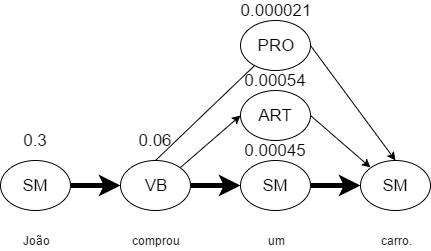
\includegraphics[height=180px]{imagens/markov2.png}
\caption{Caminhos já decididos de classificação}
\label{fig:markov2}
\end{figure}

Como visto, o método simbólico para resolver problemas de Processamento de
Linguagem Natural faz uso da criação de regras baseadas no conhecimento humano,
enquanto o método estatístico, decide através de cálculos probabilísticos
apoiados em estatísticas de um banco de dados para a resolução correta do
problema.


% Uma maneira de diferenciarmos os dois métodos é através do problema de
% ambiguidade. Por exemplo, nas frases:
%
% ``João entrou no carro conversível de óculos novos.''. E ``João entrou no carro
% conversível de farol apagado.''.
%
% Em ambas as frases, após a preposição ``de'' segue um substantivo masculino.
% Porém, cada uma das frases se refere a um substantivo diferente. A
% primeira se refere ao João, visto que não existe sentido em um carro ter óculos.
% Já a segunda se refere ao próprio carro, visto que não existe sentido em João
% ter faróis.
%
% O método simbólico para resolver esse problema faz a criação de novas regras se
% baseadas no conhecimento humano para a solução de qual o significado da frase.
% Já o método estatístico, irá verificar qual a probabilidade de cada significado
% para cada frase através de análises similares decidindo através de metódos
% estatísticos qual o significado correto para cada frase
% \cite{jacksonmoulinier2007}.

\chapter{Métodos estatísticos e simbólicos aplicados na análise de sentimentos}
\label{cap:Classificadores}

%Para o \ac{NLP} e também para o campo de estatísticas, classificadores são
%algorítmos que identificam a qual categoria determinado item pertence. Essa
%classificação é feita a partir de dados já classificados corretamente, ou seja,
%um \textit{training set}.

\section{Naive Bayes}

O Naive Bayes é um método estatístico para a classificação o qual podemos
aplicar para a análise de sentimento. Ele faz uso do teorema de Bayes para
que a partir de um \textit{training set} se possa inferir uma classificação.

Por exemplo, precisamos determinar se a seguinte frase demonstra um sentimento
negativo ou positivo: ``This place is great.'', como este método faz uso de um
\textit{training set} para a classificação, será considerado o seguinte \textit{training set} hipotético:

\begin{table}[htb]
\centering
\begin{tabular}{|l|l|}
\hline
Texto  & Categoria \\ \hline
The food was great  & Positiva     \\ \hline
They are horrible!    & Negativa     \\ \hline
I love the food here  & Positiva     \\ \hline
This place is wonderful  & Positiva     \\ \hline
Forgettable experience  & Negativa     \\ \hline
\end{tabular}
\caption{\textit{Training Set}}
\label{tab:trainingsetnb}
\end{table}

A partir do \textit{training set} representado pela tabela
\ref{tab:trainingsetnb} o método irá calcular a probabilidade da frase ``This
place is great'' ser positiva e também a possibilidade dela ser uma frase
negativa e a partir dessas duas possibilidades, será escolhida a maior.


\subsection{Teorema de Bayes}

Para cálcular a probabilidade da frase ``This place is great'' pertencer a cada categoria
utilizando o teorema da Bayes, é aplicada a seguinte equação:

\[ P(c|d)
=
\frac{P(d|c) \times P(c)}{P(d)}
\]
\[ P(Positiva|\textit{This place is great})
=
\frac{P(\textit{This place is great}|Positiva) \times
P(Positiva)}{P(\textit{This place is great})}
\]
\[ P(Negativa|\textit{This place is great})
=
\frac{P(\textit{This place is great}|Negativa) \times
P(Negativa)}{P(\textit{This place is great})}
\]


\begin{itemize}
  \item P(c$\vert$d) é a probabilidade de \textbf{d} pertencer a classe
  \textbf{c}. Ou seja, a probabilidade de \textit{``This place is great''} ser
  uma frase positiva ou negativa.
  \item P(d$\vert$c) é a probabilidade da classe \textbf{c} ser \textbf{d}. Ou
  seja, dentre todas as frases negativas ou positivas, a probabilidade de
  uma frase ser \textit{``This place is great''}.
  \item P(c) é a probabilidade da classe \textbf{c}. Ou seja, a frequência que
  frases negativas ou positivas aparecem em nosso \textit{training
  set}.
  \item P(d) é a probabilidade de \textbf{d}. Ou seja, a frequência que
  a frase \textit{``This place is great''} aparece em nosso \textit{training
  set}.
\end{itemize}

Como ambas as equações, para cálculo da probabilidade de ser negativa e positiva
tem como divisor a frase que estamos classificando, a comparação entre as
classificações é realizada através de:
\[ P(Negativa|\textit{This place is great})
=
P(\textit{This place is great}|Negativa) \times
P(Negativa)
\]
\[ P(Positiva|\textit{This place is great})
=
P(\textit{This place is great}|Positiva) \times
P(Positiva)
\]

Porém, a frase \textit{``This place is great''} não existe no
\textit{training set} tornando sua probabilidade 0.

\subsection{\textit{Naive}}

O método \textit{Naive Bayes} surge para solucionar o problema anterior,
aonde se torna díficil obter um \textit{training set} com inúmeras frases
já classificadas tornando o resultado do cálculo de probabilidade como 0.

Bayes como visto, é relacionado com o teorema utilizado para cálculo da
probabilidade, já a palavra \textit{naive}, ou ingênuo é relacionado com sua
outra característica, que é a
independência entre atributos. Esses, para o aprendizado de máquina, são
características da informação que estamos classificando. Por exemplo, ao efetuar uma classificação relacionada com medicina, atributos que seriam considerados poderiam ser histórico de doença, altura da pessoa e peso. No caso da análise de sentimentos, os atributos
são as próprias palavras do texto, ou seja, em sua classificação, ele ignora a
ordem das palavras e somente considera a frequência na qual elas aparecem.
Portanto para o \textit{Naive Bayes}:
\[ P(\textit{This place is great}|Positiva) =\]\[ P(\textit{This}|Positiva) \times
P(\textit{place}|Positiva) \times P(\textit{is}|Positiva) \times
P(\textit{great}|Positiva)
\]

Aonde que, por exemplo, P(\textit{This}$\vert$Positiva) é a quantidade de vezes que a
palavra \textit{This} foi classificada como positiva em nosso \textit{training
set} dividido pelo total de palavras classificadas como positiva:
\[P(\textit{This}|Positiva) = 1 / 13\]

Como algumas palavras podem não existir em nosso \textit{training set}, tornando
o resultado final da multiplicação das probabilidades de cada palavra como 0, é
utilizado \textit{Laplace smoothing} para que não ocorra essa possibilidade.
Neste caso, é somado 1 a cada palavra e ao total de palavras, são somadas as
quantidades de palavras diferentes do \textit{training set}, que neste caso são
as seguintes 16 palavras distintas: \textit{``The''}, \textit{``food''},
\textit{``was"}, \textit{``great"}, \textit{``They"}, \textit{``are"},
\textit{``horrible!''}, \textit{``I"}, \textit{``love"}, \textit{``here''},
\textit{``This"}, \textit{``place"}, \textit{``is"}, \textit{``wonderful"},
\textit{``Forgettable"}, \textit{``experience"} 

Neste caso, o cálculo da probabilidade da frase de exemplo \textit{``This place
is great''} para cada classe é representado pela tabela abaixo:

\begin{table}[htb]
\centering
\renewcommand{\arraystretch}{1.5}% Spread rows out...
\begin{tabular}{lll}
\hline

Palavra & Positiva & Negativa \\ \hline
This & \large $\frac{1 + 1}{13 + 16}$ & \large $\frac{0 + 1}{5 + 16}$ \\
place & \large $\frac{1 + 1}{13 + 16}$ & \large $\frac{0 + 1}{5 + 16}$ \\
is & \large $\frac{1 + 1}{13 + 16}$ & \large $\frac{0 + 1}{5 + 16}$ \\
great & \large $\frac{1 + 1}{13 + 16}$ & \large $\frac{0 + 1}{5 + 16}$ \\
\end{tabular}
\caption{Tabela de Palavras e Probabilidades.}
\label{tab:probabilidadesnb}
\end{table}

Utilizando a tabela \ref{tab:probabilidadesnb}, o classificador irá inferir a
probabilidade da frase \textit{``This place is great''} ser classificada como
positiva ou negativa:
\[ P(Positiva|\textit{This place is great})
=
P(\textit{This place is great}|Positiva) \times
P(Positiva)
\]
\[ P(\textit{This place is great}|Positiva) = \frac{1 + 1}{13 + 16} \times
\frac{1 + 1}{13 + 16} \times \frac{1 + 1}{13 + 16} \times
\frac{1 + 1}{13 + 16} \times \frac{3}{5}
\]
\[ P(\textit{This place is great}|Positiva) = 0.138
\]

\[ P(Negativa|\textit{This place is great})
=
P(\textit{This place is great}|Negativa) \times
P(Negativa)
\]
\[ P(\textit{This place is great}|Negativa) = \frac{0 + 1}{5 + 16} \times
\frac{0 + 1}{5 + 16} \times \frac{0 + 1}{5 + 16} \times
\frac{0 + 1}{5 + 16} \times \frac{2}{5}
\]
\[ P(\textit{This place is great}|Negativa) = 0.0000021
\]

Portanto, a partir dessas duas possibilidade, utilizando o método de
classificação Naive Bayes para efetuar a análise de sentimentos, ele iria
classificar a frase ``This place is great'' como positiva por essa probabilidade
(0.138) ser maior que a probabilidade dessa frase ser negativa (0.0000021).



\section{\textit{VADER}}

O \ac{VADER} é um dicionário e classificador de sentimentos que se baseia em
regras, portanto, um método de classificação simbólico. Ele é especialmente
ajustado para funcionar em redes sociais aonde temos um contexto vago e pouca
quantidade de texto, nesse contexto, ele é extremamente eficaz, podendo se
comparar a classificação feita por humanos \cite{conf/icwsm/HuttoG14}.

Esse método faz uso de um dicionário que foi construído levando em consideração
gírias e emoticons utilizados em redes sociais. Neste dicionário as palavras
estão previamente associadas a uma polaridade de sentimento (positivo e
negativo) e intensidade em uma escala de -4 até +4, como por exemplo, a palavra
\textit{great} tem a intensidade de 3.1 e \textit{horrible} -2.5. Essa
associação foi construída utilizando o método de \textit{``wisdom of the
crowd''} aonde um grupo de pessoas atribuiu os valores para cada palavra ao
invés de somente uma pessoa especializada ou uma classificação automática
através de estatística.

Ele faz uso de cinco regras gerais:


\begin{itemize}
  \item Pontuação. O ponto de exclamação (!) aumenta a magnitude da
  intensidade sem modificar a orientação semântica. Como por exemplo,
  \textit{``This place is great!!!''} é mais intenso que \textit{``This place
  is great''}.
  \item Capitalização. Especificamente, uma palavra que é relevante para a
  análise de sentimentos, quando essa é escrita em letras maiúsculas, é
  aumentada a magnitude da intensidade do sentimento sem modificar a orientação
  semântica. Como por exemplo, na frase \textit{``This place is GREAT''}, temos
  a palavra \textit{``GREAT''} (Ótimo) que está relacionada com o sentimento
  positivo. Neste caso aonde ela está escrita em letras maiúsculas, ela é mais
  intensa que \textit{``This place is great''}.
  \item Advérbios intensificadores. Estes impactam a intensidade do sentimento
  aumentando ou diminuindo a intensidade do sentimento. Na frase \textit{``This
  place is extremelly good''} o advérbio \textit{extremelly} (extremamente)
  aumenta a intensidade do sentimento expresso pela frase (\textit{good} ou
  bom), enquanto na frase \textit{``This place is marginally good''}, a palavra
  \textit{``marginally'' ou marginalmente} acaba diminuindo a intensidade do
  sentimento expresso.
  \item A palavra \textit{``but''}. Essa palavra indica uma troca no sentimento
  da frase expressa aonde que o texto seguinte a ela expressa um sentimento mais
  dominante. Por exemplo, a frase \textit{``This place is great but today, the
  service was horrible''} convém um sentimento misto.
  \item Por fim, ao examinar as três palavras anteriores, o método consegue
  identificar 90\% dos casos aonde uma negação inverte a polaridade de um texto.
  Como por exemplo, na frase \textit{``This place isn't that great''}, a
  palavra \textit{great} demonstra um sentimento positivo, porém, ao analisar
  as três palavras anteriores \textit{``place isn't that''} encontramos uma
  negação, mudando o sentimento expresso da frase de positivo para negativo.
\end{itemize}
